\documentclass[journal,12pt,twocolumn]{IEEEtran}
\usepackage{setspace}
\usepackage{gensymb}
\singlespacing
\usepackage[cmex10]{amsmath}
\usepackage{amsthm}
\usepackage{mathrsfs}
\usepackage{txfonts}
\usepackage{stfloats}
\usepackage{bm}
\usepackage{cite}
\usepackage{cases}
\usepackage{subfig}
\usepackage{longtable}
\usepackage{multirow}
\usepackage{enumitem}
\usepackage{mathtools}
\usepackage{steinmetz}
\usepackage{tikz}
\usepackage{circuitikz}
\usepackage{verbatim}
\usepackage{tfrupee}
\usepackage[breaklinks=true]{hyperref}
\usepackage{tkz-euclide}
\usetikzlibrary{calc,math}
\usepackage{listings}
    \usepackage{color}                                            %%
    \usepackage{array}                                            %%
    \usepackage{longtable}                                        %%
    \usepackage{calc}                                             %%
    \usepackage{multirow}                                         %%
    \usepackage{hhline}                                           %%
    \usepackage{ifthen}                                           %%
  %optionally (for landscape tables embedded in another document): %%
    \usepackage{lscape}     
\usepackage{multicol}
\usepackage{chngcntr}
\DeclareMathOperator*{\Res}{Res}
\renewcommand\thesection{\arabic{section}}
\renewcommand\thesubsection{\thesection.\arabic{subsection}}
\renewcommand\thesubsubsection{\thesubsection.\arabic{subsubsection}}

\renewcommand\thesectiondis{\arabic{section}}
\renewcommand\thesubsectiondis{\thesectiondis.\arabic{subsection}}
\renewcommand\thesubsubsectiondis{\thesubsectiondis.\arabic{subsubsection}}

% correct bad hyphenation here
\hyphenation{op-tical net-works semi-conduc-tor}
\def\inputGnumericTable{}                                 %%

\lstset{
frame=single, 
breaklines=true,
columns=fullflexible
}

\begin{document}


\newtheorem{theorem}{Theorem}[section]
\newtheorem{problem}{Problem}
\newtheorem{proposition}{Proposition}[section]
\newtheorem{lemma}{Lemma}[section]
\newtheorem{corollary}[theorem]{Corollary}
\newtheorem{example}{Example}[section]
\newtheorem{definition}[problem]{Definition}
\newcommand{\BEQA}{\begin{eqnarray}}
\newcommand{\EEQA}{\end{eqnarray}}
\newcommand{\define}{\stackrel{\triangle}{=}}

\bibliographystyle{IEEEtran}
\providecommand{\mbf}{\mathbf}
\providecommand{\pr}[1]{\ensuremath{\Pr\left(#1\right)}}
\providecommand{\qfunc}[1]{\ensuremath{Q\left(#1\right)}}
\providecommand{\sbrak}[1]{\ensuremath{{}\left[#1\right]}}
\providecommand{\lsbrak}[1]{\ensuremath{{}\left[#1\right.}}
\providecommand{\rsbrak}[1]{\ensuremath{{}\left.#1\right]}}
\providecommand{\brak}[1]{\ensuremath{\left(#1\right)}}
\providecommand{\lbrak}[1]{\ensuremath{\left(#1\right.}}
\providecommand{\rbrak}[1]{\ensuremath{\left.#1\right)}}
\providecommand{\cbrak}[1]{\ensuremath{\left\{#1\right\}}}
\providecommand{\lcbrak}[1]{\ensuremath{\left\{#1\right.}}
\providecommand{\rcbrak}[1]{\ensuremath{\left.#1\right\}}}
\theoremstyle{remark}
\newtheorem{rem}{Remark}
\newcommand{\sgn}{\mathop{\mathrm{sgn}}}
\providecommand{\abs}[1]{\left\vert#1\right\vert}
\providecommand{\res}[1]{\Res\displaylimits_{#1}} 
\providecommand{\norm}[1]{\left\lVert#1\right\rVert}
\providecommand{\mtx}[1]{\mathbf{#1}}
\providecommand{\mean}[1]{E\left[ #1 \right]}
\providecommand{\fourier}{\overset{\mathcal{F}}{ \rightleftharpoons}}
\providecommand{\system}{\overset{\mathcal{H}}{ \longleftrightarrow}}
\newcommand{\solution}{\noindent \textbf{Solution: }}
\newcommand{\cosec}{\,\text{cosec}\,}
\providecommand{\dec}[2]{\ensuremath{\overset{#1}{\underset{#2}{\gtrless}}}}
\newcommand{\myvec}[1]{\ensuremath{\begin{pmatrix}#1\end{pmatrix}}}
\newcommand{\mydet}[1]{\ensuremath{\begin{vmatrix}#1\end{vmatrix}}}
\numberwithin{equation}{subsection}
\makeatletter
\@addtoreset{figure}{problem}
\makeatother

\let\StandardTheFigure\thefigure
\let\vec\mathbf
\renewcommand{\thefigure}{\theproblem}



\def\putbox#1#2#3{\makebox[0in][l]{\makebox[#1][l]{}\raisebox{\baselineskip}[0in][0in]{\raisebox{#2}[0in][0in]{#3}}}}
     \def\rightbox#1{\makebox[0in][r]{#1}}
     \def\centbox#1{\makebox[0in]{#1}}
     \def\topbox#1{\raisebox{-\baselineskip}[0in][0in]{#1}}
     \def\midbox#1{\raisebox{-0.5\baselineskip}[0in][0in]{#1}}

\vspace{3cm}


\title{Assignment 1}
\author{Jaswanth Chowdary Madala}





% make the title area
\maketitle

\newpage

%\tableofcontents

\bigskip

\renewcommand{\thefigure}{\theenumi}
\renewcommand{\thetable}{\theenumi}


\begin{enumerate}
\item The base of an equilateral triangle with side $2a$ lies along the $y$-axis such that the mid-point of the base is at the origin. Find vertices of the triangle.
\begin{figure}[ht]
\centering
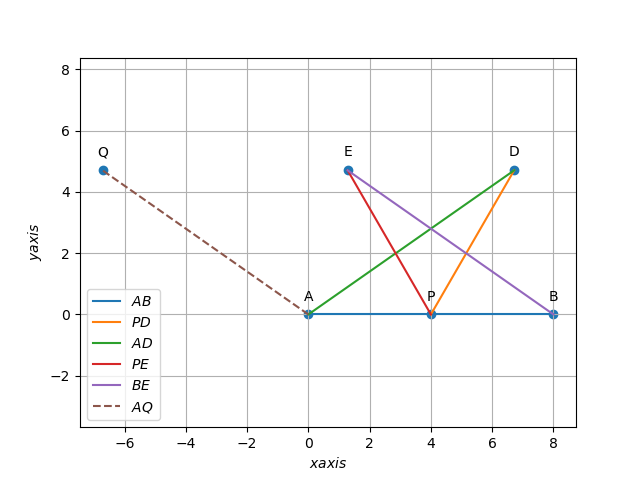
\includegraphics[width = \columnwidth]{"./figs/fig.png"}
\caption{Graph}
\label{fig:1}
\end{figure}

\textbf{Solution:}
Let the points of triangle be $\vec{A}, \vec{B}, \vec{C}$, the base $BC$ be along the $y$-axis.
\begin{align}
\vec{B} = \myvec{0\\y_1},\, \vec{C} = \myvec{0\\y_2} 
\end{align} 
Given that mid point of the base is at origin, this gives
\begin{align}
\frac{\vec{B}+\vec{C}}{2} &= 0\\
\vec{B} &= -\vec{C}\\
y_1 &= -y_2
\end{align}
Given the side length is $2a$, this gives
\begin{align}
\norm{\vec{A}-\vec{B}} = \norm{\vec{B}-\vec{C}} &= \norm{\vec{C}-\vec{A}} = 2a\\
\norm{\vec{B}-\vec{C}} &= 2a\\
\norm{\vec{B}-\brak{-\vec{B})}} &= 2a\\
\norm{\vec{B}} &= a\\
y_1 = a,\, y_2 &= -a\\
\vec{B} = \myvec{0\\a},\, \vec{C} &= \myvec{0\\-a} 
\end{align}
Let the point $\vec{A}$ be
\begin{align}
\vec{A} &= \myvec{x\\y}\\
\norm{\vec{A}-\vec{B}}^2 &= \norm{\vec{A}-\vec{C}}^2\\
\myvec{x & y-a}\myvec{x \\ y-a}&= \myvec{x & y+a}\myvec{x \\ y+a}\\
x^2 + \brak{y-a}^2 &= x^2 + \brak{y+a}^2\\
y &= 0\\
\norm{\vec{A}-\vec{B}}^2 &= \brak{2a}^2\\
\myvec{x & -a}\myvec{x \\ -a}&= 4a^2\\
x^2 + a^2 &=  4a^2
\end{align}
\begin{align}
x &= \pm \sqrt{3}a
\end{align}
The vertices of the triangle are either
\begin{align}
\vec{A} = \myvec{\sqrt{3}a\\0},\, \vec{B} = \myvec{0\\a},\, \vec{C} = \myvec{0\\-a}
\end{align}
or
\begin{align}
\vec{A} = \myvec{-\sqrt{3}a\\0},\, \vec{B} = \myvec{0\\a},\, \vec{C} = \myvec{0\\-a} 
\end{align}
\end{enumerate}



\end{document}



